\documentclass[12pt]{article}
\usepackage[utf8]{inputenc}
\usepackage[slovene]{babel}

\usepackage{hyperref}
\usepackage{listings} % za naslovnico
\usepackage{amsthm}
\usepackage{amsmath, amssymb, amsfonts}
\usepackage{graphicx}


%\graphicspath{ {./Slike/} }
\usepackage{subcaption} % za side-by-side slike
\usepackage{caption}
\usepackage[
top    = 2.cm,
bottom = 2.cm,
left   = 2.cm,
right  = 2.cm]{geometry}

\usepackage{footnote}
\usepackage{hyperref}
\hypersetup{
    colorlinks=true,
    linkcolor=blue,
    filecolor=magenta,      
    urlcolor=cyan
    }

\makesavenoteenv{tabular}
\title{Domača naloga - 1.del \\
\large Časovne vrste}

\begin{document}
    
\author{Vito Rozman}
\date{\today}
\maketitle



\section{Predstavitev uporabljenih metod}

Pri iskanju njaboljšega modela napovedovanje časovnih vrst sem testiral različne 
vrste rekurenčnih nevronskih mrež (RNN). Najprej sem začel z navadnim
RNN, ki smo ga zgradili na vajah. Model imam eno skrito stanje, ki služi spominu 
preteklih primerov. Nato sem testiral model kjer je uporabljena GRU celica,
ta nam omogoča da se model dinamično odloča kaj naj si zapomne in
kaj naj pozabi.
Na zadnje še nevronsko mrežo z imenom Long short-term memory (LSTM), ki 
omogoča uporabo kratkoročnega spomina in dolgoročnega spomina 
za grajenje prihodnjih napovedi.
LSTM model se je izkazal za najboljšega. 

Pri samih podatkih sem poizkusil več možnih pretvorb za boljše učenje.
\begin{itemize}
    \item Navadni podatki
    \item Diference med dnevi  (število novo ukuženih)
    \item Logaritmična skala števila ukuženih 
    \item Skalirane podatke z MinMaxScaler
\end{itemize}
Najblši pristop je bil skaliranje podatkov z MinMaxScaler, kar sem tudi
ugotovil pri iskanju modelov, ki že obstajajo za napovedovanje okuženih.
Za LSTM je priporočljivo da so podatki med $-1$
in $1$ zaradi vrat ki nastopajo v arhitektiri za prepust novih podatkov
in pozabo prejšnjih.

\section{Učenje, testiranje in izbira modela}

Model sem učil na skaliranih podatkih za vsako mesto posebaj. Najprej sem 
naredil učno zanko čez vseh $800$ dni potem pa še testno
čez vse dni. Uporabil se pristip s šaržami (ang. batch), kar pomeni da sem ob 
vzvratnem posodabljanju uteži najprej izračunal napako za primere v šarži
in šele na to posodobil uteži. Dan pristop se je izkazal za veliko boljše in
hitrejše kot brez šarž. V spodnji tabeli so navedeni hiperparameri ki sem jih 
preizkusil za izbran model in izbiro parametra za vsakega
od modelov napovedovanja ($7$ dni oz. $30$ dni).

\begin{center}
    %\captionof{table}{Nastavitev orodja}
    %\caption{Nastavitve orodja}
    \begin{tabular}{|c|c|c|c|}
        \hline
        \textbf{Hiperparameter} & \textbf{Prostor hiperparametrov} &  \textbf{M=7} & \textbf{M=30}\\
        \hline
        \textbf{N} & $\{7,10,14,20,30,40\}$ & $20$ & $30$\\
        \hline
        \textbf{epoch} & $\{10,100\}$ & $100$ & $100$\\
        \hline
        \textbf{batch} & $\{8,16,32,64, 128\}$ & $32$ & $32$\\
        \hline
        \textbf{hiden size} & $\{20,32,64\}$ & $32$ & $64$\\
        \hline
        \textbf{learning rate} & $\{0.1,0.01,0.001,0.0001\}$ & $0.001$ & $0.001$\\
        \hline
    \end{tabular}
\end{center}

\begin{figure}[htbp]
   
  \centering
  \begin{subfigure}[b]{0.49\textwidth}
    \centering
    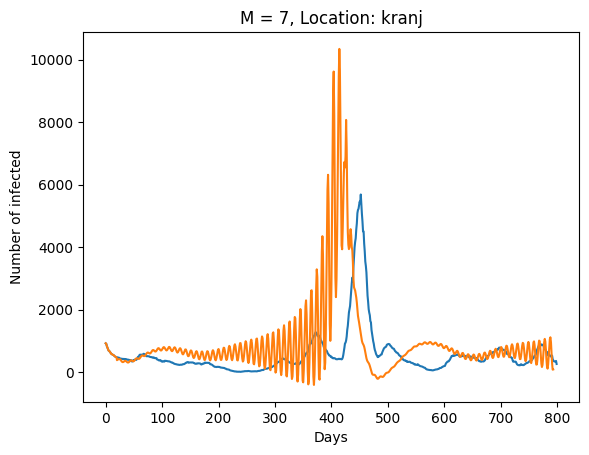
\includegraphics[width=\textwidth]{Fig/bestM7.png}
    \caption{Njaboljša napoved}
    \label{subfig:1}
  \end{subfigure}
  \hfill
  \begin{subfigure}[b]{0.49\textwidth}
    \centering
    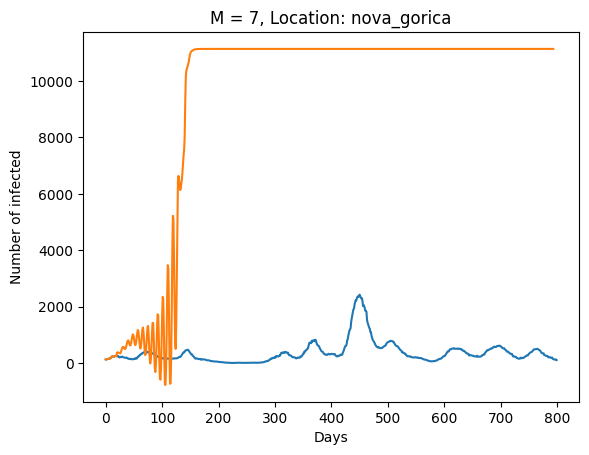
\includegraphics[width=\textwidth]{Fig/worseM7.png}
    \caption{Najslabša napoved}
    \label{subfig:2}
  \end{subfigure}
  \caption{Napovedi modela}
  \label{slika1}

\end{figure}

Ko sem računal napako modela na testni in na učni množici
sem uporabil MSE (Mean squared error).
Čudno se mi je zdelo, da je napak za napodev $7$ dni tako velika v primerjavi 
z napako za $30$ dni, kljub temu, da izgledajo grafi napovedi za $7$ dni  
veliko bolje. Na sliki \ref{slika1} je izris napovedi modela (z oranžno) in 
prava vrednost okuženih (modra). Kot njabolša napoved se je izkazala pri občini
Kranj, najslabš pa občina Nova gorica. Na sliki \ref{slika2} je izris 
povrečne napake odvisnosti od oddaljenosti napovedi.

\begin{figure}[htbp]
    \centering
    \begin{subfigure}[b]{0.49\textwidth}
        \centering
        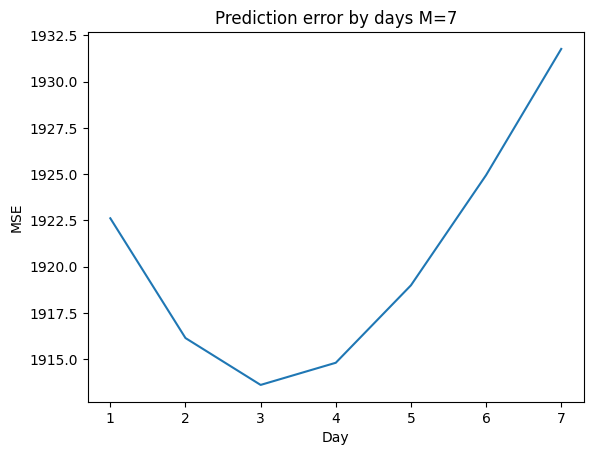
\includegraphics[width=\textwidth]{Fig/daysM7.png}
        \caption{Povprečni \textbf{MSE:} $1920.414$}
    \end{subfigure}
    \hfill
    \begin{subfigure}[b]{0.49\textwidth}
        \centering
        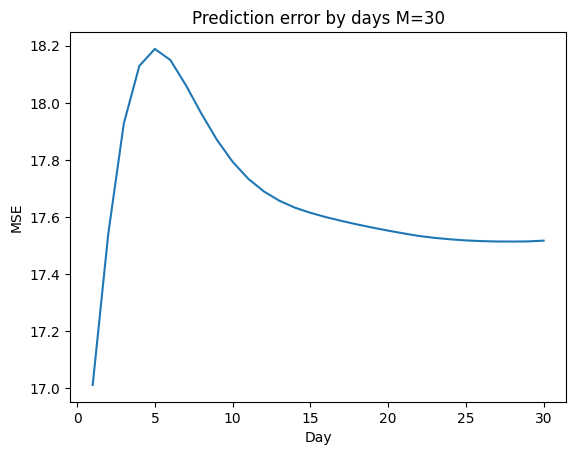
\includegraphics[width=\textwidth]{Fig/daysM30.png}
        \caption{Povprečni \textbf{MSE:} $17.668$}
    \end{subfigure}
    \caption{Napaka modele glede na oddaljenost napovedi}
    \label{slika2}

  \end{figure}



\textbf{Možne izboljšave}\\
Za grajenje boljšega modela bi lahko sestavil model ki bi napovedoval 
vse občine hkrati, ali pa vsako zaporedje vhodnih primereov pridobil
iz drugega kraja. Torej šarže bi generirla iz vsakega kraja takao da bi vsaka 
šarža vsebovala $12$ vhodni zaporedij za učenje. 
Tako bi model ob posodobitvi videl več primernih primerov.


\end{document}